\section{Benchmarking}\label{sec:bench}
%
Benchmarking was introduced in \linbox for several reasons. It would give the
user a user-friendly way for producing nice graph with no necessary knowledge
of the graphing library \gnuplot%
%
%
\footnote{\url{http://www.gnuplot.info/}}
%
or provide \linbox website with automatic new tables/graphs.
It would be used for regression testing.
It can be used for selecting default method, threshold. (cite atlas and?)
\par
%
XXX needs introductory bench references\\
XXX BTL\footnote{\url{http://projects.opencascade.org/btl/}}/eigen
%
\danger dave benchmark formats
%
\subsection{Graph/Table creation}
%
XXX data/plot structure of abstraction (update code 6.1 with new plot structure)
%
\par
%
% \begin{figure}[htbp]
	\centering
	\small
	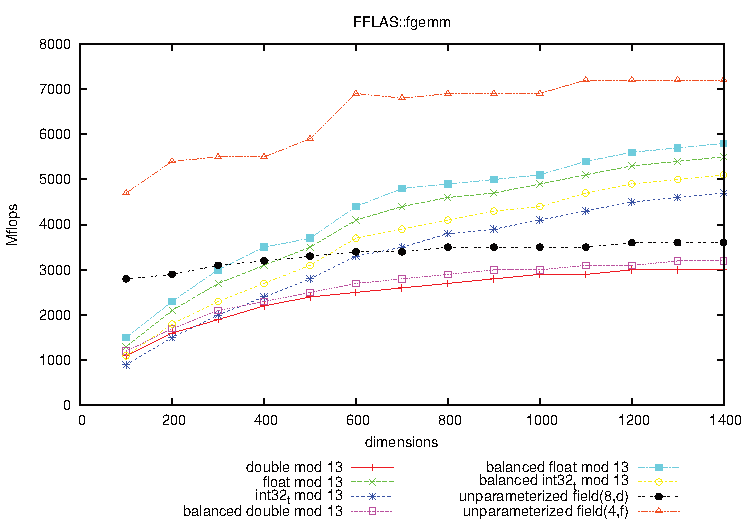
\includegraphics[scale=0.6]{Boyer_Brice/fgemm_square_13_ok}
	\caption{Example of \texttt{benchmark}: \texttt{fgemm}.\label{fig:bench}}
\end{figure}


%
XXX Time spent on each data is limited (will not start execution if fit (linear least squares) forecasts 'too long'.\\
XXX Adapts to the environment.
%
\subsection{Regression Testing}
%
XXX Tests are supposed to be comparable: regression testing.\\
XXX howto.
%
\subsection{Method Selecting}
%
XXX Default are provided, method can be selected via a benchmark (cf wino\_threshold)\\
XXX howto
